\chapter{Teorie: Obecný popis cloudu}

\section{Novinka jménem cloud computing}
V poslední době se čím dál tím více začíná mluvit o cloud computingu. Jedná se o nový typ hostingu a ukládání webového obsahu vůbec. Oproti klasickému způsobu, kde máme jeden konkrétní server, na určeném místě, se svojí danou pamětí, procesorem a pevným diskem, nám tento nový přístup umožňuje nezabývat se hardwarem, ale mluvíme takto o platformě. 

Definice se značně různí, takže použiji verzi Národního institutu standardů a technologií (National Institute of Standards and Technology) \cite{nist-cloud},
která volně přeložena zní: cloud computing je způsob poskytování sdílených škálovatelných zdrojů (výpočetní kapacita, uložiště, služby, aplikace, ...), k nímž je přistupováno skrz síť a které jsou uživateli k dispozici ihned na vyžádání. 

Mezi hlavní výhody je považováno snižování nákladů a zvyšování efektivity. Nemusíme vlastnit hardware, za jehož pořízení a správu je potřeba vynaložit nemalé finanční náklady, přičemž většina zdrojů není plně zatížena. Zvyšování efektivity se projevuje hlavně placením jen za využité zdroje. Pokud bychom měli vlastní infrastrukturu, tak v době nižší aktivity nevyužíváme možnosti serverů naplno a platíme vlastně za nevyužité zdroje. Naopak v cloudu jsou naše prostředky sdíleny s ostatními a v době neaktivity můžou být nabídnuty někomu jinému.

\section{Infrastructure as a Service, Platform as a Service, Software as a Service}
Existují různé nabídky cloudových řešení pro efektivní využívání zdrojů hardware pro více apliací. Nejzákladnější je Iaas - Infrastructure as a Service (Infrastruktura jako Služba) - jedná se například o Amazon EC2 \cite{amazon-ec2} cloud, kde platíme jen za spotřebované zdroje, které reálně využijeme a na hardware si můžeme sami instalovat co potřebujeme. 

U PaaS - Platform as a Service  (Platforma jako Služba) již nemáme přístup k hardwaru, to znamená že nelze instalovat žádný software, ale máme zde připravená API pro různé služby které můžeme využívat a většinou i další nástroje pro vývoj na lokálním stroji a pro deployment.

Nejvíce jsme od fungování služby odstíněni u SaaS - Software as a Service (Software jako Služba) - jedná se například o online e-mailové služby jako \verb|gmail.com| anebo \verb|seznam.cz|, obrázkové galerie jako \verb|flickr.com| anebo \verb|rajce.cz|, tedy služby které používáme prostřednictvím internetu a nezajímá nás jak a kde jsou data uložena a nemáme ponětí jak jsou naprogramované.

\begin{figure}[h]
\begin{center}
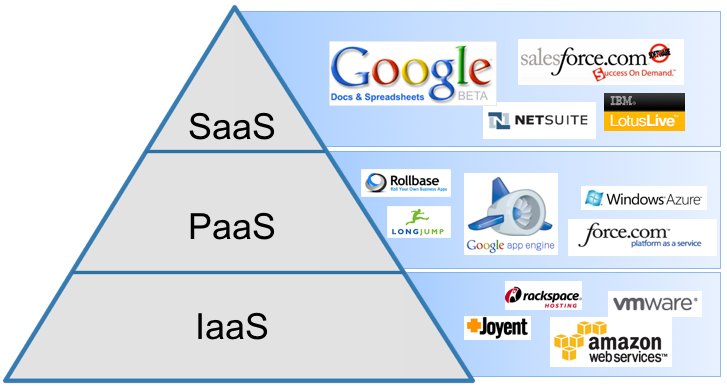
\includegraphics[width=3.5in]{figures/iaas-paas-saas.png}
\caption{Iaas, PaaS, SaaS}
\label{fig:iaas-paas-saas}
\end{center}
\end{figure}

\section{Horizontální a vertikální škálování}
Nové služby a především sociální sítě s rychlým nárůstem uživatelů a potřebě dynamicky měnit počet serverů donutily programátory a správce přemýšlet o novém způsobu ukládání a organizace dat. Pokud náš server nestíhá, tak máme dvě možnosti, jak tento problém řešit. Prvním z řešení je vertikální škálování, to znamená že koupíme silnější hardware, přidáme procesor, paměť a další komponenty podle potřeby. Nevýhodou tohoto řešení ale je, že takto nejde infrastruktura rozšiřovat do nekonečna, protože po čase narazíme na hardwarové limity. 

\begin{figure}[h]
\begin{center}
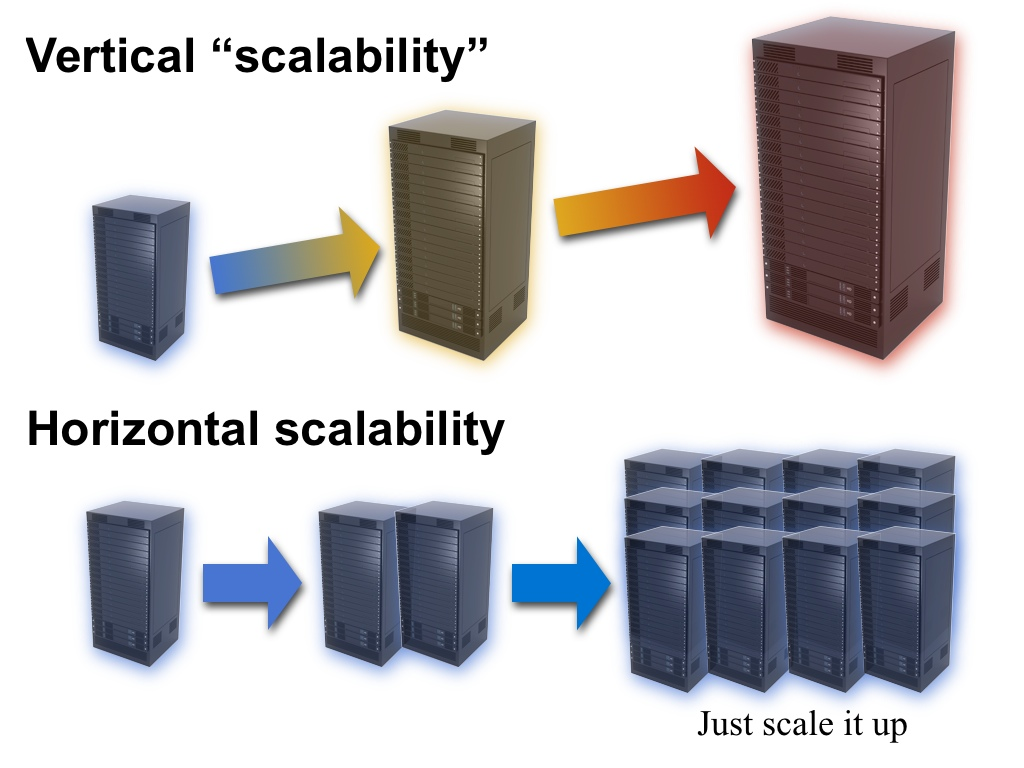
\includegraphics[width=3.5in]{figures/horizontal-vertical-scalability.jpeg}
\caption{Horizontální a vertikální škálovatelnost}
\label{fig:horizontal-vertical-scalability}
\end{center}
\end{figure}

Druhou z možností je nakoupení více serverů. Nemusí být ani velmi výkonné, ale řešení spočívá v propojení těchto počítačů dohromady, címž můžeme zvětšovat naši infrastrukturu bez omezení. Můžeme toto řešení přirovnat k problému z běžného života, kdy potřebujeme převézt určitý počet osob z jednoho místa na druhé. Můžeme objednat autobus, který jednoduše řeší tento problém. Pokud počet osob naroste, tak můžeme objednat autobus s větší kapacitou, jenže pokud se bude počet osob zvyšovat, tak časem již nenajdeme tak velký autobus pro přepravu všech osob. Takže jako řešení budeme muset objednat více vozidel, ale ty poté budeme moci efektivně zaplňovat podle počtu osob. Nevýhoda tohoto řešení spočívá v složitějším správě infrastruktury, potřebujeme software, který se stará o propojení, synchronizaci a spolupráci všech částí systému, nebo pokud nějáký stroj přestane fungovat, musíme zajistit aby ho ihned zastoupil jiný se stejnou funkcí jako předchozí.

Pro cloud computing se obecně vžila značka mraku (v angličtině znamená cloud mrak) a vznikla proto, že na obrázcích a schématech se ve většině případů mrakem značí internet a vzdálená zařízení, které nejsou uloženy u nás. A to právě z toho důvodu, že jsou tyto služby většinou přístupné skrze internet a přistupujeme k nim vzdáleně.

\section{Různé druhy pohledu na cloud computing}
Cloud computing se jako každá jiná novinka potýkal s různými názory od těch pozitivních až po ty negativní. Někteří tvrdili, že se jedná jen o buzzword\footnote{módní slovo}, který má nalákat nové zákazníky, jiní predikovali, že se takovýto princip nemůže nikdy uchytit. Zde je pár výroků  z doby, kdy nebyl tolik rozšířený:

\begin{quotation}
The interesting thing about Cloud Computing is that we’ve redefined Cloud Computing to include everything that we already do...  I don’t understand what we would do differently in the light of Cloud Computing other than change the wording of some of our ads.

\em Larry Ellison, Oracle Corporation CEO, Wall Street Journal, 26. září 2008
\end{quotation}

Larry Ellison říká, že cloud computing je jen pojmenování toho, co již dávno používáme a že jediná změna, která je potřeba je změna textů u reklam. Je pravda, že některé velké společnosti, jako třeba Oracle anebo Google používali tento přístup již mnohem dříve než vzniknul samotný název, ale pravdou je, že v posledních dvou letech se začal cloud computing používat masivněji a to hlavně díky možnosti pronájmu cloudů. Nyní si mohou programátoři vyzkoušet pracovat s cloudy a použít je i pro své menší aplikace, bez nutnosti spravovat a starat se o velké množství strojů.

\begin{quotation}
A lot of people are jumping on the (cloud) bandwagon, but I have not heard two people say the same thing about it. There are multiple definitions out there of “the cloud.”

\em Andy Isherwood, HP’s vice president, ZDnet News, 11. prosinec 2008
\end{quotation}

Andy Isherwood naznačuje, že není přesně daná definice toho, co ještě cloud je a co již není. Je to způsobeno tím, že po vzniku tohoto názvu chtěl každý s více než jedním serverm označovat svoje služby jako cloudové. To vedlo spíše ke zmatení, ale v poslední době se toto slovní spojení ustálilo pro farmu serverů se snadnou škálovatelností a jednoduchou možností přidat novou instanci.

\begin{quotation}
It’s stupidity. It’s worse than stupidity: it’s a marketing hype campaign. Somebody is saying this is inevitable — and whenever you hear somebody saying that, it’s very likely to be a set of businesses campaigning to make it true.

\em Richard Stallman, Founder of GNU Project and Free Software Foundation, The Guardian, 29. září 2008
\end{quotation}

Richard Stallman má na cloud poněkud negativní názor a pro The Guardian vyslovil názor že se jedná o hloupost a jde jen o nafouknutou bublinu podpořenou businessovými kampaněmi. Kritizoval hlavně uložení dat mimo naši vlastní kontrolu a nutnost spolehnutí se na společnost, které dávame naše data a aplikace k dispozici. Nikdo nám nemůže na sto procent zaručit, že bude tato společnost fungovat i po několika letech. Navíc jsme většinou vázáni na API rozhraní, služby a možnosti platformy určené danou společností.

Pokud budeme chtít přenést službu k jinému poskytovateli cloudu, bude nám to s největší pravděpodobností činit nemalé potíže, v angličtině se používá termín \emph{lock-in}, což znamená doslova zamknutí. Sice v poslední době vznikají návrhy na jednotná rozhraní a sjednocení rozhraní těchto služeb, aby byl přechod co nejjednodušší, ale ty se bohužel zatím nesetkaly s větším rozšířením. Do budoucna by to mohla být jedna z klíčových vlastností při rozhodování, kterou službu zvolit.

\section{Porovnání Amazon Web Services, Windows Azure a Google App Engine}
Největší konkurenti Google App Engine jsou Amazon Web Services - EC2 (Elastic Compute Cloud) a Microsoft Azure. Pokud budemem mít zakázku, pro kterou je nejvýhodnější použit cloudovou infrastrukturu, budeme se pravděpodobně rozhodovat mezi těmito třemi, jedná se o velké a známé společnosti s rozsáhlým zázemím. Je tedy málo pravděpodobné, že by ze dne na den přestaly provozovat svoje služby, což může být velký problém u menších nebo méně znamých společnotí.

\subsection{Amazon Web Services - Elastic Compute Cloud}
Amazon EC2 je spíše blíže modelu IaaS, takže dostaneme hardware s kterým si můžeme dělat co chceme, instalovat libovolný software a musíme si ho sami spravovat. Největší výhodou je rychlé přidávání nových serverů kdykoliv potřebujueme a platba jen za spotřebované zdroje. Navíc není tento cloud vázán žádnými API a omezeními, takže pokud budeme chtít přesunout naši aplikaci na náš server, tak nebudeme muset měnit aplikaci a to platí i naopak, tedy pro přesun aplikace na cloud. Jedná se čistě o pronájem hardwaru. Neýhoda Amazon Web Services je v tom, že platíme hned jakmile nahrejeme naši aplikaci, neexistují žádné volné kvóty jako u App Engine. Amazon v rámci svých služeb nabízí i další možnosti, například speciální relační i nerelační uložiště a další produkty, celý seznam je možné najít na stránce \verb|http://aws.amazon.com/products/|. 

\subsection{Microsoft Azure}
Microsoft Azure je již více podobný App Engine, jedná se o PaaS, máme zde již připravené prostředí pro několik jazyků: .NET (C\# a VisualBasic), C++, PHP, Ruby, Python a Java. Výhodou je, že můžeme použít klasickou relační databázi nazvanou SQL Azure Database (SAD), což se vyplatí pokud migrujeme nějaký projekt postavený na relační databázi, ale tento typ je hůře škálovatelný. Vedle SAD můžeme použít i Azure Storage, která osahuje nerelační tabulky, tabulky pro velké objemy dat (blobs) a fronty (queues). Azure má speciální staging prostředí, kde můžeme přímo na cloudu vyvíjet aplikaci a nedostane se k ní nikdo, dokud není připravena na spuštení. V tomto prostředí také můžeme spouštět aplikaci v debug režimu, což nám umožňuje například nastavovat breakpointy, pokud potřebujeme aplikaci ladit přímo na cloudu. Azure také umožňuje propojení s Microsoft Live službami a s vývojovým prostředím Microsoft Visual Studio. Stejně jako u Amazonu platíme ihned jakmile nasadíme aplikaci do plného provozu, aby ji mohli vidět i ostatní. Azure je určitě výhodné použít, pokud vyvíjíme aplikace v technologiích od Microsoftu, naše infrastruktura je na těchto tehcnologiích založena anebo pokud používáme jako vývojový nástroj Visual Studio.

\subsection{Google App Engine}
Oproti dvěma předchozím má App Engine hlavní výhodu v tom, že nemusíme platit ihned jak aplikaci nahrajeme na cloud. Jsou zde nastavené kvóty, které jsou velmi vysoké a je potřeba velká návštěvnost pro jejich přesáhnutí, což je pro začínající aplikaci výhodné obzvláště v České republice. Takže pokud začínáme se startupem, nemusíme se v počátcích obávat velkých investic a pokud bude náš projekt úspěšný a bude obsluhovat velký počet požadavků, tak poté budeme muset platit jen za přesáhnuté limity, které se každých 24~hodin vynulují. Některé limity jsou nastaveny napevno a nejdou zvýšit ani za poplatek, je to kvůli tomu, aby se nemohlo stát, že jedna aplikace zaneprázdní celý cloud, což by mělo za následek zpomalení i ostatních aplikací. Tyto limity jsou naštěstí velmi vysoké, například datastore API má maximálně 141~241~791 volání za den a 784~676 volání za minutu.  zde je přehledná tabulka kvót a omezení. Kvóty se průběžně navyšují, takže tato data jsou  platná pro květen 2011 \ref{tab:quotas}.

\begin{table}[h]
\centering
\caption{Tabulka kvót a ceny}\label{tab:quotas}
\begin{tabular}{|l|l|}
   \hline
     Služba & Omezení \\
   \hline
    Procesorový čas & 6.5 hodny / den \\
    Odchozí data & 1 GB / den \\
    Přijatá data &1 GB / den \\
    Uložená data v Datastore & 1 GB \\
    Počet indexů v Datastore & 200 \\
    Volání Mail API & 7~000 / den \\ 
    Příjemců mailu & 2~000 \\
    Volání URL Fetch API & 657~084 \\
    URL Fetch API odeslaná data  & 4 GB / den \\
    URL Fetch API přijatá data  & 4 GB / den \\
    Volání XMPP API & 46~310~400 / den \\
    XMPP API odeslaná data & 1~046 GB / den \\
    Pdeslané XMPP zprávy & 46~310~400 / den \\
    Poslaných XMPP pozvánek & 100~000 / den \\
    Volání Channel API & 46~310~400 / den \\
    Vytvořených Channel spojení & 8~640 / den \\
    Channel API odeslaná data & 1~046  GB / den \\
    Volání Task Queue API & 100~000 / den \\
    Uložených úkolů & 1~000~000 /den \\
    Velikost uložených úkolů & 1 GB / den \\
    Nahrání aplikací & 1~000 / den \\
   \hline
\end{tabular}
\end{table}

Standardně se aplikace nahraje na adresu jako doména třetího řádu ve
tvaru \verb|jmeno-aplikace.appspot.com| a pokud potřebujeme můžeme nastavit i doménu vlastní. Další výhodou App Engine je možnost provozovat více verzí stejné aplikace najednou. Nahrají se pak jako poddomény, takže například \verb|verze.jmeno-aplikace.appspot.cz|. Tyto verze mohou běžet na cloudu zároveň a v administraci se dá nastavit, která bude výchozí. Toto do jisté míry nahrazuje staging area z Azure, výhodou zde je, že můžeme mít libovolný počet verzí. App Engine bohužel podporuje jen jazyky Java, Python a Go\footnote{Přidání jazyka Go bylo oznámeno na konferenci Google I/O 10. května 2011}. Díky různým projektům, které jsou schopny přeložit další jazyky do javovského bytekódu, zde tedy můžeme spouštět velké množství dalších jazyků i když je to vykoupeno nižší rychlostí. Můžeme zde tedy používat jazyky jako: Groovy, Scala, Ruby s pomocí JRuby, PHP díky projektu Quercus (viz dále), JavaScript za pomoci Rhino a další. Jedním z důvodů přidání Javy do App Engine byla právě možnost běhu dalších jazyků nad Java Virtual Machine. Co se Javy týká, tak nejsou povoleny všechny třídy, nemůžeme například vytvářet nová vlákna, nemůžeme vytvářet nové soubory a některá volání třídy \verb|System| nedělají nic, například \verb|System.exit()| a \verb|Sytem.gc()|. Seznam všech povolených tříd je možné najít na adrese \verb|http://code.google.com/appengine/docs/java/jrewhitelist.html|. Kvůli těmto omezením bohužel nemůžeme použít všechny knihovny, anebo musíme použít upravenou verzi pro App Engine. Seznam nejpoužívanějších frameworků a knihoven s popisem zda jsou kompatibilní a případné nastavení pro App Engine je dostupný na adrese \verb|http://groups.google.com/group/google-appengine-java/web/will-it-play-in-app-engine?pli=1|. Na App Engine nemáme jistotu, že bude naše aplikace přímo připravena, protože kvůli tomu, aby se šetřily prostředky, jsou nahrány jen aktivní a využívané aplikace, se po určité době neaktivity aplikace odstaví a nahradí ji jiná. Můžeme si za poplatek zařídit, že naše aplikace bude vždy k dispozici, protože každé nahrání stojí čas. Můžeme tedy využívat většinu frameworků, ale kvůli tomuto nahrávání se každý kód navíc negativně projeví na době prvního přístupu k aplikaci, což je velmi znatelné především u rozsáhlých frameworků.

\section{API služby}
Abychom mohli propojit naši aplikaci s ostatními máme na App Engine velké množství API sloužících k různým účelům. Pojďme si nyní projít jaké možnosti máme. Některé z nich asi vůbec nevyužijeme, ale některé jsou velmi užitečné a důležité. Google pro vývoj aplikací nabízí pro všechny podporované jazyky SDK\footnote{Software Development Kit - sada vývojářských nástrojů určených pro speciální aplikci nebo platformu}, aktuální je nyní verze 1.5.0.1 z 16. května 2011.

Asi jednou z nejpoužívanějších služeb, pokud pomineme Datastore, je Memcache. Jedná se o možnost, jak zrychlit častý přístup do databáze. Jedná se o key-value cache, která je přibližně desetkrát až stokrát rychejší, než přístup k Datastore. Nehodí se ale pro vše, protože data z ní po vypršení zmizí. Místo klasického cachování na disk, tedy máme možnost ukládat data do paměti. Implementace je podle standardu JSR-107, takže bude kompatibilní s dalšími knihovnami.

Mezi další užitečné služby patří Mail, posílání mailů funguje klasicky pomocí tříd javax.mail. Můžeme přidávat i přílohy. Některé soubory jsou z bezpečnostních důvodů zakázány, ale všechny běžně používané jsou povoleny. Přijímání e-mailů se ošetřuje pomocí servletu\footnote{Servlet je komponenta napsaná v jazyce Java, určená pro spouštění na webovém serveru}. Ve \verb|web.xml| se nastaví servlet pro url \verb|/_ah/mail/jmeno-emailu| a e-mail má tvar: \verb|jmeno-emailu@id-aplikace.appspot.com| a to bohužel i v případě, že máme nastavenou naši vlastní doménu. Příchozí e-mail se chová jako HTTP požadavek, takže v servletu se musíme zpracování postarat sami, podle toho co potřebujeme. 

Podobně jako Mail funguje i služba pro práci s XMPP protokolem\footnote{Extensible Messaging and Presence Protocol (http://xmpp.org/about-xmpp/technology-overview/)}. Jedná se o otevřený standardizovaný protokol Jabberu postavený na XML. Princip na App Engine je podobný jako s e-mailem, identifikátor příjemce je JID, který se dá získat  z e-mailu. Podporovány jsou i další funkce, jako posílání pozvánek, nastavování statusů a další. Přijímáme pomocí servletu nastaveného na adresu: \verb|/_ah/xmpp/message/chat/|.

Kvůli absenci JMS\footnote{Java Message Service (http://en.wikipedia.org/wiki/Java\_Message\_Service)} máme na App Engine možnost použít Task Queues. Jedná se o frontu úloh, které by mohly zpomalit náš systém, takže je výhodnější je zpracovat později. Fronta funguje následovně: pomocí Task Queues API přidáme do fronty URL naší aplikace, můžeme jí předávat parametry stejně jako u klasické URL\footnote{Uniform Resource Locator (http://en.wikipedia.org/wiki/Uniform\_Resource\_Locator)}. Provedení úlohy z fronty je záležitostí servletu, na který je URL nastavena pomocí \verb|web.xml|. Vykonání úlohy je omezeno deseti minutami, toto by měl být dostatečný limit pro běžné úlohy. Pokud servlet vrátí HTTP status mimo rozmezí 200 - 299, což znamená chybu, tak se úloha zavolá znovu aby proběhla v pořádku. Pokud potřebujeme informovat aplikaci o dokončení úlohy, musíme to řešit pomocí Datastore.

Pokud potřebujeme naše stránky integrovat s nějakou webovou službou, anebo používat veřejná REST API, použijeme URL Fetch. Jedná se o klasické java.net API, můžeme použít HTTP i HTTPS, většinu běžných portů a samozřejmě i všechny HTTP metody: GET, POST, PUT, HEAD i DELETE pro správné fungování REST rozhraní. K požadavku můžeme nastavovat i vlastní HTTP hlavičky.

Na některá data, jako například obrázky, nebo velké soubory se Datastore nehodí, maximální velikost entity je 1MB. Právě kvůli tomuto účelu můžeme na App Engine použít Blobstore, jedná se o uložiště pro velké soubory do velikosti až 2GB. Blobstore je plně oddělen od Datastore. Nahrávání je velice jednoduché, stačí použít forumář s prvkem \verb|<input type=”file” />| a atribut action formuláře nastavíme pomocí \verb|<%= blobstoreService.createUploadUrl("/upload")%>|.
Blobstore už se sám postará aby se soubor nahrál na správné místo. Zobrazovat soubory můžeme pomocí \verb|blobstoreService.serve(blob-key)|, potřebujeme k tomu klíč souboru. Tato služba umí vybrat všechny uložené soubory. Práce je velmi podobná jako s Datastore, akorát s tím rozdílem, že zde pracujeme s velkými soubory. Jedná se o užitečnou službu, protože dříve než existovala tato služba, se ukládání řešilo rozdělením do mnoha samostatných entit o velikosti 1MB a při zobrazení jsme je museli zase nazpět složit. Toto všechno se dělo na aplikační úrovni, takže jsme museli ošetřit všechny chybové případy a bylo vše velmi zdlouhavé a nepohodlné. Takto se o ukládání souborů stará AppEngine sám a nám stačí jednoduché API.

S předchozím Blobstore souvisí i další služba: Images. Jedná se o možnost úpravu obrázků přímo na serveru. Obrázky se načítají z Blobstore anebo můžeme službě předat přímo pole \verb|byte[]|. Můžeme takto aplikovat jednoduché transformace jako je změna velikosti, otočení, oříznutí, skládní obrázků a také magická funkce "I’m feeling lucky", která změní nastavení tmavých a světlých barev a k tomu také zvýší kontrast obrázku, výsledkem jsou pak více barevnější obrázky. Upravené obrázky můžeme přímo posílat uživetelům anebo uložit do Blobstore, pokud se budou zobrazovat častěji. Služba obsahuje základní transformace, ale na vytvoření náhledů nebo menší úpravy jako zvětšení a zmenšení obrázku, které jsou pravěpodobně na webových stránkách nejpoužívanější, se Image API hodí výborně.

Pokud potřebujeme u naší aplikace vytvořit sekci jen pro přihlášené uživatele, nabízí nám k tomu App Engine možnost použít Users API a interní přihlašovací mechanismus Googlu využívaný u všech aplikací této společnosti, například tedy \verb|gmail.com|, \verb|youtube.com| a dalších. Použití je jednoduché, pokud uživatel není přihlášený, tak ho přesměrujeme na vygenerovanou přihlašovací stránku. Ta je stejná pro všechny služby Googlu, zadáme e-mail a heslo. Poté můžeme nastavit, které všechny údaje o sobě chceme aplikaci, do které se právě přihlašujeme, poskytnout. Nakonec nás stránka přesměruje zpět na naši aplikaci. Nyní můžeme o uživateli zjistit základní informace: přihlašovací e-mail a jednoznačný identifikátor ID. Odhlašování funguje stejně jako přihlašování, přesměrujeme uživatele na odhlašovací stránku Google, která nás následně po odhlášení znovu přesměruje, tentokrát na naši aplikaci.

Pokud chceme dát možnost přihlašování i pro uživatele, kteří nevlastní účet u Google, můžeme použít OAuth protokol. Ten není vázaný na konkrétní společnost, takže si můžeme vybrat poskytovatele. Jedná se o možnost přihlášení uživatelským jménem a heslem jiné aplikace a v naší aplikaci jen kontrolujeme token. Výhoda tohoto způsobu je, že uživateli stačí jeden účet pro více aplikací, nemusí si tak pamatovat hesla pro každou stránku na které má účet. S touto službou se pracuje velmi podobně jako s předchozím API.

App Engine obsahuje Capabilities API pomocí něhož můžeme zjistit, zda daná služba běží anebo ne. Můžeme tak ošetřit případ, kdy zrovna probíhá údržba anebo výpadek a služby jsou nedostupné. Jsou zde dostupné informace o těchto službách: Blobstore, čtení z Datastore, zápis do Datastore, Images, Mail, MemCache, TaskQueue, Url Fetch a XMPP.

Pro lepší spolupráci s klientskou stranou máme k dispozici Channel API. To se stará o trvalé spojení JavaScriptu na stránce se servery Googlu, aniž by se musel klient stále dotazovat serveru. Toto se hodí, pokud chceme uživatele informovat o nastalé akci, toto se hodí například na hry pro více hráčů a internetové chaty.

Posledním rozšířením je Multitenancy API, to nám dává možnost používat jmenné prostory pro naše data, můžeme je aplikovat na: Datastore, Memcache, Task Queue a Blobstore. Můžeme tak provozovat více oddělených stránek z jedné aplikace a pro každou stránku budeme mít speciální jmenný prostor. Data se tak nebudou překrývat a budou správně oddělena.

\section{Omezení cloudu}
Pokud se rozhodneme naši službu provozovat na cloudu, tak musíme již od návrhu počítat s jistými omezeními a odlišnou strukturou aplikace, než na jakou jsme zvyklí z klasických aplikací. Většina z těchto omezení plyne z požadavku na škálovatelnost aplikací.

Pro většinu programátorů je největším problémem databáze, používá se totiž poměrně nový typ - NoSQL databáze (pro češtinu nejlépe hodí překlad: nerelační databáze). Databáze používaná na App Engine se nazývá BigTable\footnote{http://en.wikipedia.org/wiki/BigTable}, jedná se o vícerozměrnou distribuovanou mapu optimalizovanou pro rychlé čtení a pomalejší zápis, protože u běžných aplikací je čtení dat mnohem častější operace. Google navíc toto uložiště využívá i pro své ostatní služby. Naprostá většina dnešních aplikací využívá relační databázi, pravděpodobně jednu z trojice nejpoužívanějších: Oracle, PostgreSQL, MySQL anebo MS-SQL, všechny tyto databáze mají tabulky a pomocí konstrukce JOIN je můžeme navzájem libovolně spojovat. Nevýhoda tohoto řešení ale spočívá v tom, že pro tuto operaci potřebujeme všechny tabulky, které v dotazu spojujeme. V praxi se tedy používá samostatný stroj jen pro databázi. U škálovatelných aplikací, se ale nemůžeme spolehnout na to, že jsou všechny tabulky na jednom místě, mohou totiž být v různých datacentrech na různých kontinentech. Řešením je tedy ukládání všech potřebných dat do jedné tabulky anebo přiřazování do skupin, které se budou spojovat a databáze se sama postará o to, aby byla data uložena ve stejném datacentru. App Engine proto používá speciální dotazovací jazyk šitý na míru tomuto uložišti: GQL - Google Query Language\footnote{http://code.google.com/appengine/docs/python/datastore/gqlreference.html},
což je podmnožina SQL jazyka pro App Engine Datastore. Nenajdeme v něm samozřejmě operátor JOIN a s ním spojené konstrukce.

Mezi další omezení patří žádná anebo omezená možnost vyhledávání nad sloupci databáze. Není totiž zaručeno jakou strukturu sloupců bude tabulka mít. Toto jde obejít vytvořením speciální tabulky se slovy a v kterých sloupcích se vyskytují, ale je to dosti složité a musíme se o vše starat sami. Pokud potřebujeme vyhledávat na internetové stránce, je jednodušší použít internetový vyhledávač například Google, Bing anebo český Seznam. Všechny jmenované mají nástroj pro vyhledávání podle domény, takže stačí jen přidat formulář na naše stránky. Pokud potřebujeme vyhledávát v našich interních datech budeme muset použít nějaké rozsáhlejší řešení.

\section{Vývoj pro App Engine}
Pokud se rozhodneme vytvářet naše aplikace pro App Engine, tak máme k dispozici poměrně vyspělou infrastrukturu. Google oficiálně podporuje Eclipse plugin pro App Engine\footnote{Google Plugin for Eclipse - http://code.google.com/appengine/docs/java/tools/eclipse.html},
ale dostupné jsou i plně funkční pluginy pro NetBeans IDE\footnote{NetBeans support for Google App Engine - http://kenai.com/projects/nbappengine/pages/Home}
a také pro vývojové prostředí IntelliJ IDEA\footnote{Google App Engine Integration for IntelliJ - http://plugins.intellij.net/plugin/?id=4254}. Pomocí těchto pluginů můžeme jednoduše vyvíjet aplikaci na našem domácím stroji bez nutnosti připojení k internetu. Součástí je totiž jednoduchý webový server simulující App Engine, jedná se o upravený Jetty server\footnote{Jetty je odlehčený open source HTTP server a servlet kontejner napsaný v Javě}.
Máme zde úplně stejné API jako na produkčním serveru a pomocí URL \verb|http://localhost/_ah/admin| máme k dispozici jednoduchou administraci obsahující správce Datastore, správce Task Queues a další. Data se lokálně ukládají do souboru \verb|.bin| přímo ve složce \verb|/build| projektu. Deploy na lokální prostředí je stejný jako u jakéhokoliv jiného serveru, tedy pomocí tlačítka v IDE, anebo můžeme použít některý z buildovacích nástrojů, jako například ANT anebo Maven. Pro upload přímo na produkční prostředí je možné také použít přímo plugin, stejně tak jako je integrováno tlačítko pro lokání upload, tak je zde možnost uploadu přímo na App Engine. Vše probíhá nahráním výsledného \verb|war| souboru aplikace na speciální URL. Pokud bychom chtěli integrovat nahrávání do jiného nástroje, máme možnost provést upload pomocí skriptu pro příkazovou řádku. Ten provádí upload pomocí \verb|jar| souboru, takže není problém celý deployment integrovat do naší infrastruktury. Dále můžeme mít libovolný počet verzí aplikace, všechny jsou na URL \verb|verze.jmeno-aplikace.appspot.com|, kde verze je jakýkoliv řetězec definovaný ve \verb|web.xml| a výchozí možnost se nastavuje v administraci přímo na App Enginu. Máme zde navíc oproti localhostu\footnote{označení serveru, který běží na našem lokálním počítači} mnoho různých nastavení a statistik. Pro každou aplikaci, kterých můžeme k jednomu Google účtu mít až deset je zde podrobný přehled návštěv a spotřebovaných prostředků, počet aktivních instancí, logy, přehled a správa Datastore, nastavení aplikace a další.

\section{Zajímavé aplikace}
Nyní představím zajímavé aplikace a stránky, které můžeme na App Engine cloudu najít. Nacházejí se zde zajímavé experimenty, jako například běh různých jazyků nad JVM (Java Virtual Machine) až po stránky s velkým zatížením. Nejzajímavější z nich je pravděpodobně stránka \verb|www.officialroyalwedding2011.org|, založená k příležitosti svatby anglického prince Williama a Catherine Middleton. V pátek 29. dubna, tedy v den oddání, bylo na hosting generováno 2~000 požadavků za vteřinu a dohromady bylo zobrazeno 15 milionů stránek od 5,6 milionu uživatelů. I přes tento nápor stránka běžela bez problémů a bez ovlivnění více jak 200~000 dalších aplikací běžících na stejném cloudu, které všechny dohromady za den vygenerovaly více jak 1,5 miliardy stránek. \cite{royal-wedding}

Další podobnou zkouškou pro App Engine byla aplikace Google Moderator. Tato aplikace běžela dva dny v březnu roku 2009 na stránce \verb|www.whitehouse.gov|. Jednlo se o hlasovací systém určený pro obyvatele USA, kde může kdokoliv vložit svůj dotaz a další uživatelé pak hlasují o tom, které dotazy jsou nejlepší. Vítězné otázky byly dne 29. března zodpovězeny prezidentem Barackem Obamou. Během 48 hodin zadalo 92~934 uživatelů 104~073 otázek a ohodnotilo je 3~605~984 hlasy. Při nejvyšší zátěži obsloužil App Engine 700 dotazů za vteřinu. \cite{whitehouse-app}

\begin{figure}[h]
\begin{center}
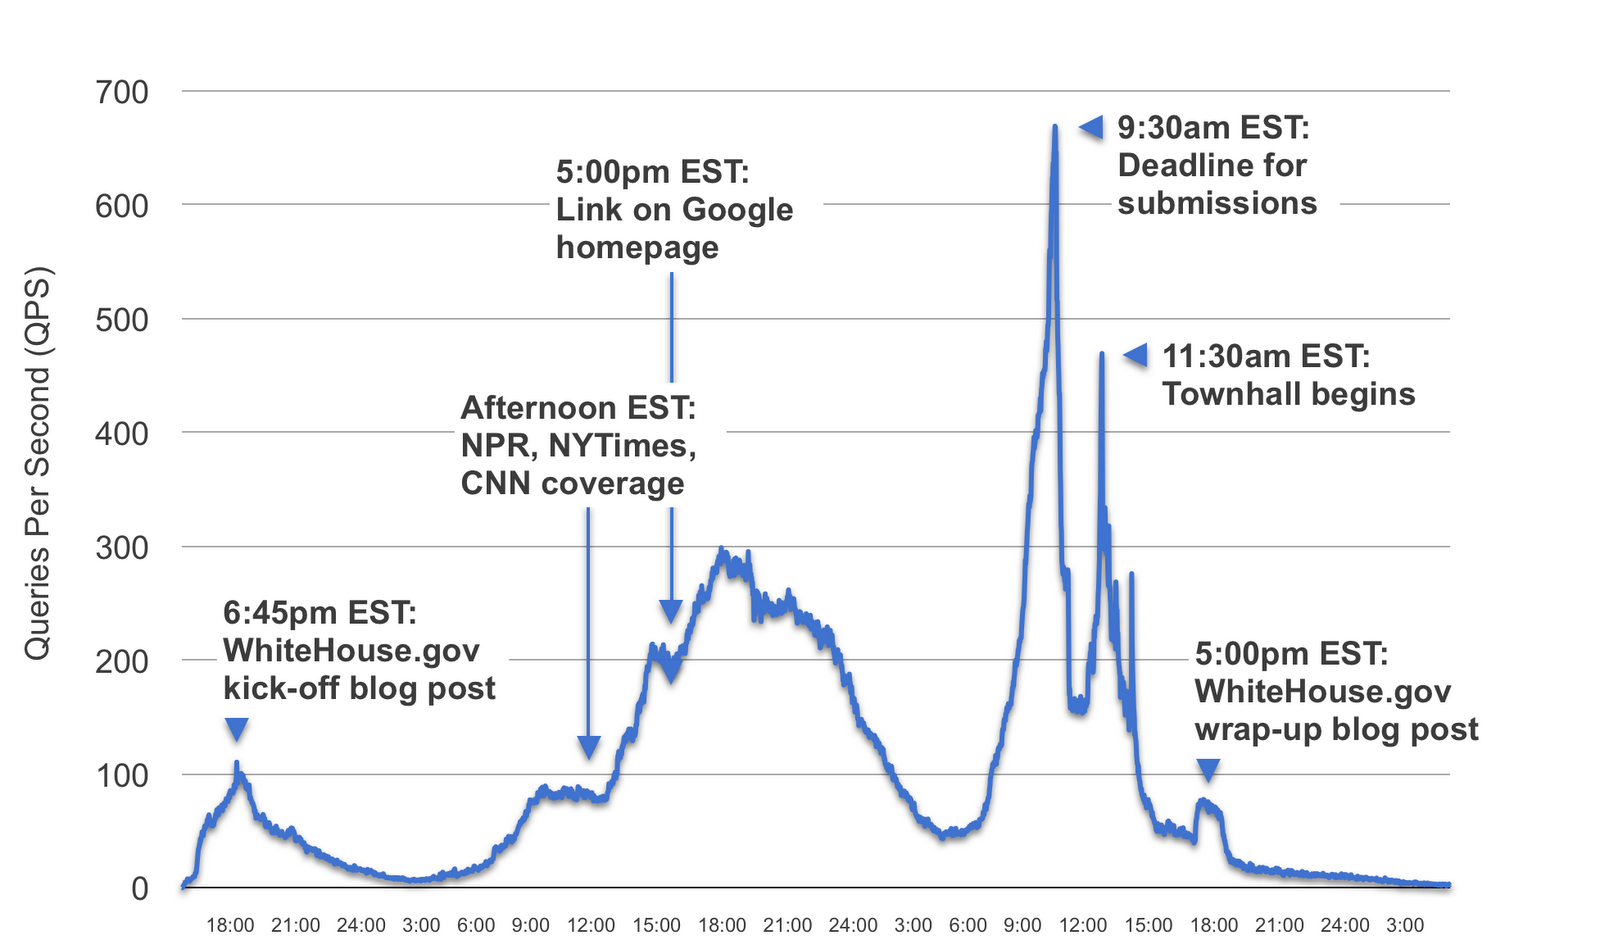
\includegraphics[width=3.5in]{figures/townhallgraphic.png}
\caption{Zatížení App Engine serverů v době spuštění aplikace Google Moderator pro Bílý Dům \cite{whitehouse-app}}
\label{fig:whitehouse-app-picutre}
\end{center}
\end{figure}

Nyní bych rád zmínil některé zajímavá a užitečné aplikace, které jsou ideálí pro umístění v cloudu. Jednou z nich je i Socialwok (\verb|www.socialwok.com|), jedná se o obdobu facebooku pro práci, můžeme zde sdílet naši práci v Google Apps (Docs, Calendar, Spreadsheet) se spolupracovníky a ti mohou do našich dokumentů zasahovat. Jedná se o zajímavou myšlenku a praktické využití sociálních sítí.

Podobnou službou je i Giftag (\verb|www.giftag.com|), ta umí uložit část webové stránky a tu pak sdílet s dalšími. Existuje doplněk pro internetové prohlížeče, který zjednoduší uložení stránky. Všechny uložené části navíc můžeme organizovat a přidávat do seznamů. Tato služba nám může pomoci, pokud pracujeme na výzkumu anebo potřebujeme udělat prezentaci na které pracuje více lidí.
 
Největší uplatnění získaly cloudy díky sociálním sítím, další služba je určena právě pro ně. Jedná se o BuddyPoke! (\verb|www.buddypoke.com|), umožňuje nám dát si na náš profil trojrozměrný obrázek postavičky s popisem jak se cítíme. Tuto aplikaci můžeme najít na všech používaných sociálních sítích, které vkládání obrázků dovolují, tedy: Facebook, Orkut, MySpace, hi5, Netlog, Ning a dalších. Tato aplikace nemá žádný přínos, ale díky velkému množství podporovaných sociálních sítí a jejich velké oblibě v poslední době je tato služba velice úspěšná.

Poslední zmíněná aplikace je naopak velmi přínosná. Mnoho vývojářů by rádo vidělo na App Engine podporu pro skriptovací jazyk PHP, ten se bohužel vývojáři v nejbližším čase přidat neplánují. Projekt Quercus (\verb|quercus.caucho.com|) umožňuje právě běh PHP na JVM a vývojáři připravili speciální verzi pro App Engine, kde můžeme spouštět PHP s podporou některých Java frameworků.

Další zajímavé a úspěšné projekty jsou na stránce: \verb|http://code.google.com/appengine/casestudies.html|

\section{Budoucnost cloudů}
Cloud je zcela nová možnost hostování webových aplikací. Jedná se o novinku, a tak bude nějáký čas trvat, než se společnosti a vývojáři přizpůsobí. Vývoj cloudových aplikací je dost odlišný a proto je potřeba přizpůsobit vývojový cyklus apliakcí již od samého začátku. Je důležité poznamenat, že rozhodně ne všechny typy aplikací jsou pro cloud vhodné. Je tedy třeba rozhodnout, kdy se cloud vyplatí a kdy naopak ne. Důležité bude také sledovat, které velké společnosti budou cloud podporovat a jaké budou možnosti v nabídce cloudových hostingů. Je dobré vědět, že například Google s podporou cloudů do budoucnosti počítá a hodlá je dál rozšiřovat i do dalších sfér. Na každoroční konferenci \emph{Google I/O}, která se letos konala 10. a 11. května 2011 v San Franciscu\footnote{Google I/O 2011 - http://www.google.com/events/io/2011/index-live.html}, představil Google funkční prototyp takzvaného Chromebooku \footnote{Chromebook - http://www.google.com/chromebook/}. Jedná se o notebook s operačním systémem Chromium OS\footnote{Chromium OS - http://www.chromium.org/chromium-os}, je optimalizován pro používání webu a rychlou práci s ním. Všechny aplikace jsou jednoduše webové stránky, odpadají tak problémy se synchronizací, novými verzemi a podobně. Nevýhoda tohoto přístupu je, že pokud se ocitneme bez internetu, tak nám nepůjde žádná aplikace. Myslím, že toto je dobrá záruka pro využití cloudových aplikací do budoucna a je třeba se přizpůsobit tomuto trendu do budoucna.
